\chapter{FUNDAMENTAÇÃO CONCEITUAL E TRABALHOS RELACIONADOS}

\section{Canais e subconjuntos de informação}

Considere uma tarefa de classificação supervisionada em que cada observação é representada por um vetor padronizado
\begin{equation}
  X=(X_1,\ldots,X_d),
  \label{eq:input-vector}
\end{equation}
no qual cada componente $X_j$ corresponde a um canal de informação. O rótulo da observação é denotado por $Y\in\{1,\ldots,K\}$, sendo $K$ o número de classes.

O termo canal enfatiza a origem informacional da variável, e não apenas sua posição em uma tabela. Em um sistema de monitoramento, $X_j$ pode ser a resposta de um sensor. Em uma aplicação clínica, pode ser uma medida fisiológica ou um resultado laboratorial. Em outros contextos, pode corresponder a um atributo derivado, a um registro administrativo ou a uma avaliação humana. Dois canais diferentes podem inclusive compartilhar a mesma infraestrutura de produção, aspecto que será relevante para a discussão de custos.

Seja
\begin{equation}
  I\subseteq\{1,\ldots,d\}
\end{equation}
um conjunto de índices. O subconjunto de canais correspondente é
\begin{equation}
  S_I=\{X_i:i\in I\}.
  \label{eq:subset-si}
\end{equation}
O índice $I$ é escrito em letra maiúscula porque representa um conjunto de índices, e não um identificador escalar. Um classificador treinado com $S_I$ observa apenas as coordenadas de $X$ pertencentes a esse subconjunto.

Para $d$ canais, existem
\begin{equation}
  2^d-1
  \label{eq:nonempty-subsets}
\end{equation}
subconjuntos não vazios. Essa enumeração cresce exponencialmente, mas é viável nos cenários estudados: cinco canais produzem 31 subconjuntos e sete canais produzem 127. A avaliação exaustiva evita que a análise dependa de uma ordem arbitrária de inclusão e permite comparar configurações de mesma cardinalidade. A Figura~\ref{fig:conceito-reticulado} ilustra a diferença com um exemplo de três canais: enquanto uma cadeia prefixada avalia apenas uma sequência aninhada de subconjuntos, a enumeração exaustiva percorre todo o espaço de combinações.

\begin{figure}[H]
  \centering
  \caption{Cadeia prefixada de dimensões e enumeração exaustiva de subconjuntos}
  \label{fig:conceito-reticulado}
  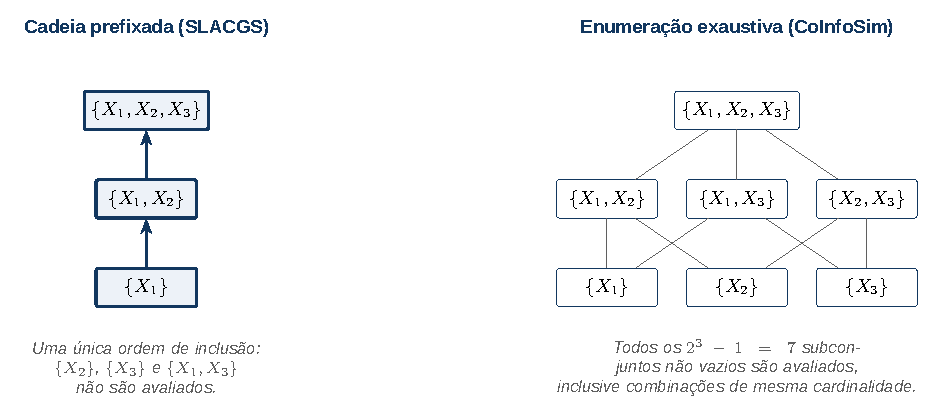
\includegraphics[width=0.92\textwidth]{figures/conceptual/reticulado_subconjuntos.pdf}
  \sourcebelow{elaboração própria}
\end{figure}

\section{Cooperação, complementaridade e redundância}

A literatura de seleção de variáveis distingue relevância individual de utilidade conjunta. Uma variável pode conter informação sobre $Y$ quando analisada isoladamente e, ainda assim, ser dispensável na presença de outra variável que carrega informação semelhante. De modo inverso, uma variável com desempenho marginal modesto pode melhorar significativamente um classificador quando complementa um canal mais forte. \textcite{guyon2003} destacam que variáveis relevantes podem ser redundantes e que a avaliação de subconjuntos é necessária para capturar dependências que um ranking marginal não revela. Trabalhos de seleção informacional também modelam explicitamente o equilíbrio entre relevância para o alvo, redundância e complementaridade condicional \cite{brown2012}.

Neste relatório, três noções são separadas:

\begin{description}
  \item[Relevância marginal:] capacidade de um canal contribuir para a classificação quando observado isoladamente;
  \item[Redundância:] sobreposição de informação útil entre canais, de forma que a inclusão conjunta produz ganho pequeno ou nulo;
  \item[Complementaridade:] contribuição adicional que emerge da combinação, ainda que um dos canais seja fraco individualmente.
\end{description}

A cooperação é observada quando um subconjunto produz menor perda que configurações mais simples em determinado regime amostral. Essa definição é operacional: ela não exige atribuir causalidade aos canais nem interpretar a cooperação como interação física entre sensores. O termo indica uma vantagem de classificação associada ao uso conjunto das informações. A Figura~\ref{fig:conceito-cooperacao} resume as três noções em um exemplo com quatro canais: um canal informativo isoladamente, um par redundante e um canal que só se torna útil em combinação.

\begin{figure}[H]
  \centering
  \caption{Relações informacionais entre canais e alvo: relevância, redundância e complementaridade}
  \label{fig:conceito-cooperacao}
  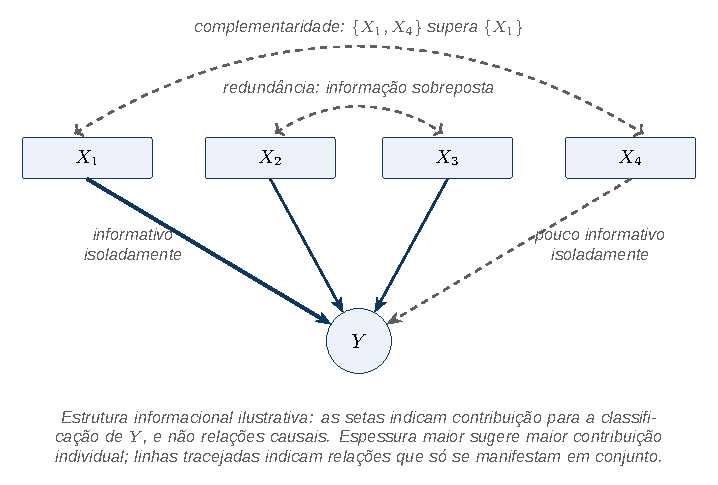
\includegraphics[width=0.80\textwidth]{figures/conceptual/cooperacao_canais.pdf}
  \sourcebelow{elaboração própria}
  \notailustracao{O esquema é uma estrutura informacional ilustrativa e não representa um modelo causal dos dados.}
\end{figure}

A formulação se relaciona a métodos \emph{wrapper} de seleção de variáveis (\textit{feature selection}), nos quais um modelo preditivo avalia subconjuntos candidatos. Contudo, o objetivo do \CoInfoSim{} é diferente de selecionar uma única configuração final. A seleção convencional costuma procurar um subconjunto que maximize uma função de desempenho sob um protocolo de validação. O \CoInfoSim{} acompanha a organização de todos os subconjuntos ao longo de $n$, produzindo rankings, relações par a par e limiares de transição. Assim, o objeto de interesse é uma trajetória estrutural, e não apenas a solução ótima em um único tamanho amostral.

Essa distinção também altera a interpretação de eficiência. A coincidência exata do melhor subconjunto pode ser instável quando duas configurações possuem perdas quase iguais. Para decisões operacionais, pode ser mais informativo saber se um subconjunto menor vence consistentemente diversos concorrentes, se uma família de configurações permanece próxima do topo e em que faixa de $n$ uma combinação maior passa a oferecer vantagem. Por essa razão, o trabalho preserva métricas complementares, em vez de reduzir a estrutura a um único vencedor.

\section{Dimensionalidade e pequenas amostras}

A inclusão de canais cria uma tensão entre informação potencial e dificuldade de estimação. Em um cenário ideal, um classificador com acesso a mais variáveis poderia ignorar qualquer informação inútil. Em amostras finitas, porém, os parâmetros, fronteiras e dependências precisam ser estimados. O aumento da dimensão amplia o espaço de hipóteses e pode elevar a variância do modelo.

O estudo clássico de \textcite{hughes1968} analisou a acurácia média de reconhecedores estatísticos em função do número de medidas e do tamanho da amostra de treinamento. Esse resultado é frequentemente associado ao \emph{peaking phenomenon}: em determinadas condições, adicionar dimensões melhora inicialmente o desempenho, mas, para um tamanho amostral fixo, a dificuldade de estimação pode superar o ganho informacional. \textcite{raudys1991} sistematizam efeitos de pequenas amostras e apresentam recomendações práticas para reconhecimento estatístico de padrões.

O \CoInfoSim{} investiga uma manifestação relacionada, mas não idêntica. Em vez de aumentar apenas a dimensão por uma sequência prefixada, compara subconjuntos diferentes. Uma dupla pode superar um canal isolado somente após determinado tamanho amostral; uma tripla pode precisar de ainda mais dados; e subconjuntos de mesma cardinalidade podem trocar de posição conforme o classificador aprende dependências específicas.

Seja $f$ um classificador e $n$ o número de amostras de treinamento por classe. A perda média de um subconjunto $S_I$ será denotada por
\begin{equation}
  \overline{L}_{S_I,f}(n).
  \label{eq:mean-loss-foundation}
\end{equation}
A dependência explícita em $n$ é essencial. Não se trata apenas de registrar o desempenho final, mas de observar como as curvas se aproximam, se cruzam e eventualmente se estabilizam. A cooperação pode surgir quando a informação adicional de um subconjunto maior passa a compensar seu custo estatístico de aprendizagem.

O fenômeno não deve ser interpretado como uma lei segundo a qual o melhor canal isolado sempre vence em pequenas amostras ou subconjuntos maiores sempre vencem no limite. A forma das curvas depende da distribuição, do classificador, do ruído e das relações entre canais. O valor da análise experimental está precisamente em não impor previamente essa ordenação.

\section{Treinamento sintético e avaliação em dados reais}

Dados sintéticos podem ser avaliados sob diferentes critérios. Uma avaliação puramente distributiva compara estatísticas, densidades, projeções ou distâncias entre dados reais e gerados. Uma avaliação orientada à tarefa verifica se amostras sintéticas sustentam modelos úteis em uma aplicação real. \textcite{esteban2017} propõem, entre outras estratégias, treinar um modelo supervisionado em dados sintéticos e testá-lo em dados reais, protocolo conhecido como \emph{Train on Synthetic, Test on Real}.

O desenho do \CoInfoSim{} adota a mesma direção geral, mas amplia o objeto avaliado. Os dados reais de treinamento são usados para ajustar um modelo gerador condicional à classe. Esse gerador produz as amostras sintéticas de treinamento usadas para treinar os classificadores, enquanto a avaliação ocorre sobre o mesmo conjunto de teste real fixo, que não participa do ajuste do gerador. Para cada dataset são comparados três braços:
\begin{align}
  &\RealToReal,\label{eq:arm-real}\\
  &\GaussianToReal,\label{eq:arm-gaussian}\\
  &\GMMToReal.\label{eq:arm-gmm}
\end{align}

No primeiro braço, o treinamento também utiliza amostras reais de treinamento balanceadas. Nos demais, o treinamento dos classificadores utiliza amostras sintéticas de treinamento produzidas por modelos geradores ajustados exclusivamente aos dados reais de treinamento. O teste é compartilhado pelos três braços. Essa escolha reduz uma fonte de variação: as diferenças observadas não decorrem de conjuntos de avaliação distintos.

Uma comparação Synthetic$\rightarrow$Real convencional pode ser resumida por uma métrica de desempenho de um único modelo. No \CoInfoSim{}, cada braço produz uma família de curvas indexada por subconjunto, classificador e tamanho amostral. A pergunta deixa de ser apenas ``o treinamento sintético prediz bem?'' e passa a incluir ``o treinamento sintético preserva as relações entre configurações de canais?''.

Essa mudança permite separar três tipos de fidelidade:

\begin{description}
  \item[Fidelidade geométrica:] proximidade visual ou estatística entre a distribuição real e a distribuição gerada;
  \item[Fidelidade preditiva absoluta:] proximidade das perdas absolutas obtidas por treinamento real e sintético;
  \item[Preservação do \PredictiveCooperationProfile:] preservação da ordenação, das relações efetivas de vencedor e da dinâmica de inversões entre subconjuntos.
\end{description}

Os três tipos podem se relacionar, mas nenhum implica automaticamente os demais. Essa separação será retomada na análise dos resultados, especialmente nos cenários Occupancy e SUPPORT2.

\section{Perfil de cooperação preditiva}

O \PredictiveCooperationProfile{} é a representação quantitativa de como o desempenho preditivo relativo dos subconjuntos de canais evolui ao longo do tamanho amostral, para um dataset, um classificador e uma condição de treinamento determinados. Ele é definido a partir das curvas de perda média estimada dos subconjuntos e organizado em três níveis analíticos crescentes de detalhe:

\begin{enumerate}
  \item a \textbf{ordenação global} dos subconjuntos em cada $n$, comparável por correlação de ranking;
  \item a \textbf{relação efetiva de vencedor par a par}, que resume, para cada par de subconjuntos, qual deles tem menor perda estimada em cada $n$, com uma regra explícita de propagação sob empate exato;
  \item a \textbf{dinâmica de inversões}, isto é, os momentos em que a relação efetiva de vencedor de um par troca de sentido ao longo do tamanho amostral.
\end{enumerate}

É importante distinguir o perfil de um \PredictiveCooperationPattern{}: o perfil é o objeto quantitativo --- a série de rankings, matrizes de vencedores e matrizes de inversões ao longo de $n$ --- enquanto um padrão é uma regularidade interpretada a partir de um ou mais perfis, como "pares redundantes raramente invertem" ou "o vencedor entre duas famílias de subconjuntos se estabiliza cedo". O relatório reporta perfis diretamente e discute padrões apenas como leitura interpretativa desses perfis, nunca como o dado bruto.

Esses três níveis possuem sensibilidades diferentes. Uma correlação de ranking elevada pode coexistir com uma discordância de vencedor em pares específicos. Uma relação de vencedor pode ser idêntica entre duas condições mesmo que os regimes amostrais em que ela se estabilizou sejam distintos. A dinâmica de inversões, por sua vez, decompõe-se em duas perguntas logicamente separadas: os mesmos pares invertem (uma questão de \emph{existência}) e, entre os pares que invertem em ambas as condições, as inversões ocorrem em tamanhos amostrais semelhantes (uma questão de \emph{regime amostral})? Essas duas perguntas geram dois indicadores distintos, nunca combinados em um único índice.

A preservação do perfil de cooperação preditiva é, portanto, multidimensional. O trabalho não procura declarar que um braço "preservou" ou "não preservou" por meio de uma única medida. Em vez disso, compara:

\begin{enumerate}
  \item a ordenação global dos subconjuntos ($\rankrho$);
  \item as relações efetivas de vencedor entre pares (\WinnersAgreement, $\AW$);
  \item a existência de inversões válidas de vencedor (\ReversalExistenceAgreement, $\AR$);
  \item o regime amostral das inversões compartilhadas (\ReversalSampleSizeSimilarity, $\SR$).
\end{enumerate}

As definições formais e os procedimentos de cálculo são apresentados no Capítulo 6.

\section{Modelos geradores}

\subsection{Gaussiana única por classe}

O modelo sintético mais simples considera uma distribuição normal multivariada para cada classe:
\begin{equation}
  X\mid Y=c \sim \mathcal{N}(\mu_c,\Sigma_c),
  \qquad c=1,\ldots,K.
  \label{eq:class-gaussian}
\end{equation}
Nos cenários ancorados, a Gaussiana de cada classe é ajustada no espaço padronizado a partir dos dados reais de treinamento: $\widehat{\mu}_c$ e $\widehat{\Sigma}_c$ correspondem, respectivamente, à média e à covariância amostrais calculadas nesses dados reais de treinamento. As matrizes de covariância podem diferir entre classes.

A Gaussiana única resume cada classe por um centro e uma estrutura global de dispersão e correlação. Sua capacidade de representar assimetrias, caudas, multimodalidade e regiões desconectadas é limitada. Essa limitação, contudo, não a torna cientificamente desinteressante. O modelo é leve, interpretável e permite perguntar quanto da estrutura cooperativa depende apenas de momentos de primeira e segunda ordem.

Se os classificadores treinados com amostras da Gaussiana única reproduzirem ranking e relações de vitória quase tão bem quanto aqueles treinados com amostras de um gerador mais flexível, isso constitui um resultado favorável ao modelo simples. Em estudos de simulação, simplicidade reduz custo de parametrização, facilita inspeção dos parâmetros e pode abrir espaço para análises teóricas posteriores. Por essa razão, a comparação com GMM não é tratada como uma competição em que a maior flexibilidade deve necessariamente vencer.

\subsection{Mistura de gaussianas}

Uma mistura gaussiana representa a distribuição de cada classe por uma combinação ponderada de componentes:
\begin{equation}
  p(x\mid Y=c)
  =
  \sum_{k=1}^{K_c}\pi_{ck}
  \mathcal{N}(x\mid\mu_{ck},\Sigma_{ck}),
  \label{eq:gmm}
\end{equation}
em que $\pi_{ck}\geq 0$, $\sum_k\pi_{ck}=1$ e $K_c$ é o número de componentes da classe $c$. Misturas finitas constituem uma família flexível para representar heterogeneidade e multimodalidade \cite{mclachlan2000}.

No protocolo implementado, um GMM é ajustado separadamente para cada classe no espaço completo dos canais, usando apenas os dados reais de treinamento. A parametrização de cada candidato é obtida por máxima verossimilhança, e o número de componentes é selecionado pelo menor BIC. Esse critério combina a log-verossimilhança maximizada com uma penalização pela quantidade de parâmetros \cite{schwarz1978}, buscando evitar que a flexibilidade cresça sem controle.

O GMM pode aproximar formas visuais que uma única elipse gaussiana não representa. Ainda assim, maior fidelidade geométrica não garante maior preservação do perfil de cooperação preditiva. A divisão dos dados em componentes pode melhorar a representação global da densidade sem preservar exatamente as regiões que determinam as fronteiras de um classificador ou as diferenças relativas entre subconjuntos. Essa possibilidade será importante no Occupancy, em que o GMM parece reproduzir melhor a forma dos dados, mas a Gaussiana única apresenta indicadores de preservação ligeiramente superiores em determinadas configurações finais.

\section{Classificadores}

O conjunto de classificadores foi escolhido para produzir contrastes entre hipóteses de aprendizagem, mantendo o protocolo computacionalmente viável.

\subsection{Linear SVM}

O Support Vector Machine linear procura um hiperplano de separação associado a uma margem entre as classes \cite{cortes1995}. A versão linear preserva continuidade com o simulador anterior e oferece um modelo sensível à geometria global do espaço padronizado. Sua simplicidade favorece a execução repetida em todos os subconjuntos e tamanhos amostrais.

\subsection{Regressão logística}

A regressão logística modela a probabilidade condicional da classe por uma função logística de uma combinação linear dos canais. Trata-se de um baseline probabilístico amplamente utilizado, cuja interpretação e estimação são bem estabelecidas \cite{hosmer2013}. Embora compartilhe uma fronteira linear com o Linear SVM, o critério de ajuste é diferente, permitindo verificar se a preservação estrutural depende do mecanismo de aprendizagem.

\subsection{Gaussian Naive Bayes}

O Gaussian Naive Bayes supõe independência condicional entre canais dada a classe e modela distribuições marginais gaussianas. Apesar da hipótese forte, classificadores Naive Bayes podem apresentar bom desempenho mesmo quando a independência não é estritamente satisfeita \cite{handyu2001}. No contexto do \CoInfoSim{}, o modelo é particularmente informativo porque permite contrastar ganhos associados à acumulação de evidências marginais com ganhos que dependem de relações multivariadas.

\subsection{Random Forest}

Random Forest combina múltiplas árvores construídas sob aleatoriedade de amostras e de variáveis, agregando suas previsões \cite{breiman2001}. O classificador introduz não linearidade e interações que não estão disponíveis aos modelos lineares. Em contrapartida, seu custo computacional é substancialmente maior em um protocolo que exige centenas de ajustes para cada subconjunto, tamanho amostral e replicação.

Por essa razão, o Random Forest não integra uma comparação simétrica entre todos os datasets nesta versão do trabalho. Ele foi incorporado como estudo adicional no SUPPORT2, com calibração realizada apenas nos dados reais de treinamento e configuração congelada para todos os braços. O resultado deve ser interpretado como evidência específica da interação entre esse classificador, o SUPPORT2 e os geradores avaliados, e não como demonstração de superioridade geral.

As implementações utilizadas pertencem ao ecossistema scikit-learn, cuja arquitetura e conjunto de algoritmos são descritos por \textcite{pedregosa2011}.

\section{Custos operacionais}

A ligação entre cooperação e custos aparece em duas etapas. A primeira, realizada neste trabalho, caracteriza a organização dos subconjuntos: quais combinações vencem, como se ordenam e quando passam a superar alternativas mais simples. A segunda, futura, atribuirá custos específicos a essas configurações e formulará decisões sob restrições operacionais.

A taxonomia de \textcite{turney2002} mostra que aprendizagem sensível a custos pode incluir custos de erro, de testes, de intervenção, de aquisição de casos e de computação, entre outros. Para canais de informação, uma modelagem de domínio pode considerar:

\begin{itemize}
  \item custos fixos de compra, instalação e certificação;
  \item custos recorrentes de manutenção, calibração e substituição;
  \item custos variáveis de energia, comunicação e armazenamento por amostra;
  \item tempo, latência e disponibilidade operacional;
  \item risco, invasividade ou desconforto associado à coleta;
  \item trabalho de especialistas;
  \item infraestrutura compartilhada entre canais;
  \item custo de produção do rótulo ou da referência.
\end{itemize}

O problema de seleção de sensores sob restrições possui literatura própria, com formulações baseadas em otimização e valor informacional \cite{joshi2009,krause2008}. O \CoInfoSim{} ainda não resolve esse problema. Sua contribuição atual é produzir os objetos necessários para uma extensão orientada a custos.

A modelagem econômica deverá respeitar a unidade real de decisão. Em um exame que produz várias variáveis, o custo pode estar associado ao procedimento, e não a cada canal separadamente. Em uma rede de sensores, parte do custo é fixa e parte depende da taxa de coleta. Em uma auditoria, o custo pode ser por documento, por lote ou por hora de especialista. O rótulo $Y$ pode ser obtido imediatamente ou exigir acompanhamento posterior. Portanto, uma expressão aditiva simples pode ser utilizada como exemplo didático, mas não deve ser confundida com uma definição universal.

A motivação de custos permanece, contudo, cientificamente conectada aos indicadores de preservação do perfil. Um ranking preservado permite comparar famílias de configurações; a \WinnersAgreement{} resume relações par a par relevantes para substituir ou eliminar alternativas; e a matriz de inversões $\Rmat$ indica em que regime amostral uma configuração mais complexa passou a superar outra. Essas informações precedem qualquer otimização monetária e ajudam a formular o problema de decisão adequado a cada domínio.
